\section{Aufbau und elektronische Beschaltung}
In Abbildung \eqref{fig:Aufbau} ist der schematische Aufbau des gesamten Gerätes aufgezeigt. Allerdings sind die Kühlung und die Blei-Burg für den Detektor und den Vorverstärker nicht eingezeichnet. Das Ziel des Aufbaus ist es einen Spannungsimpuls zu erzeugen der proportional zu der deponierten $\gamma$-Energie ist. Die benötigten Komponenten werden im folgenden beschrieben.

\begin{figure}[H]
  \centering
  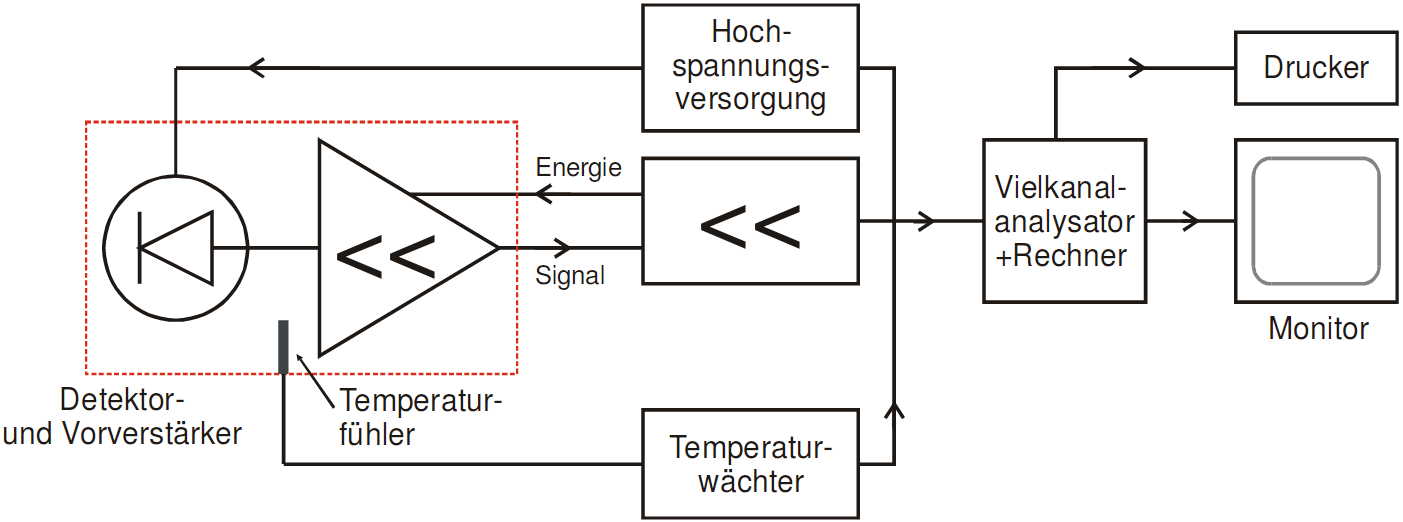
\includegraphics[width=\linewidth]{Bilder/Aufbau.png}
  \caption{Der schematische Aufbau des $\gamma$-Spektrometers ohne Kühlung \cite{V18}.}
  \label{fig:Aufbau}
\end{figure}

\textbf{Detektor:} \\
Der verwendete Detektor ist in Abbildung \eqref{fig:DetektorAufbau} skizziert. Der Germanium-Kristall hat die Gestalt eines Hohlzylinders und ist von außen mit Lithium bedampft und von innen mit Gold beschichtet. Dadurch ist der Kristall außen n-dotiert und innen p-dotiert. Der Pluspol für die Sperrspannung wird an der Lithium-Schicht angebracht. \\
Um den Kristall befindet sich eine Schutzhaube aus Aluminium. Diese schließt den Kristall luftdicht ein, dadurch kann der Kristall nicht verunreinigt werden. Allerdings können wegen der Schutzhaube und der Lithium-Schicht nur $\gamma$-Energien größer als 40\,keV nachgewiesen werden.
\todo{und E>150keV?}
\begin{figure}[H]
  \centering
  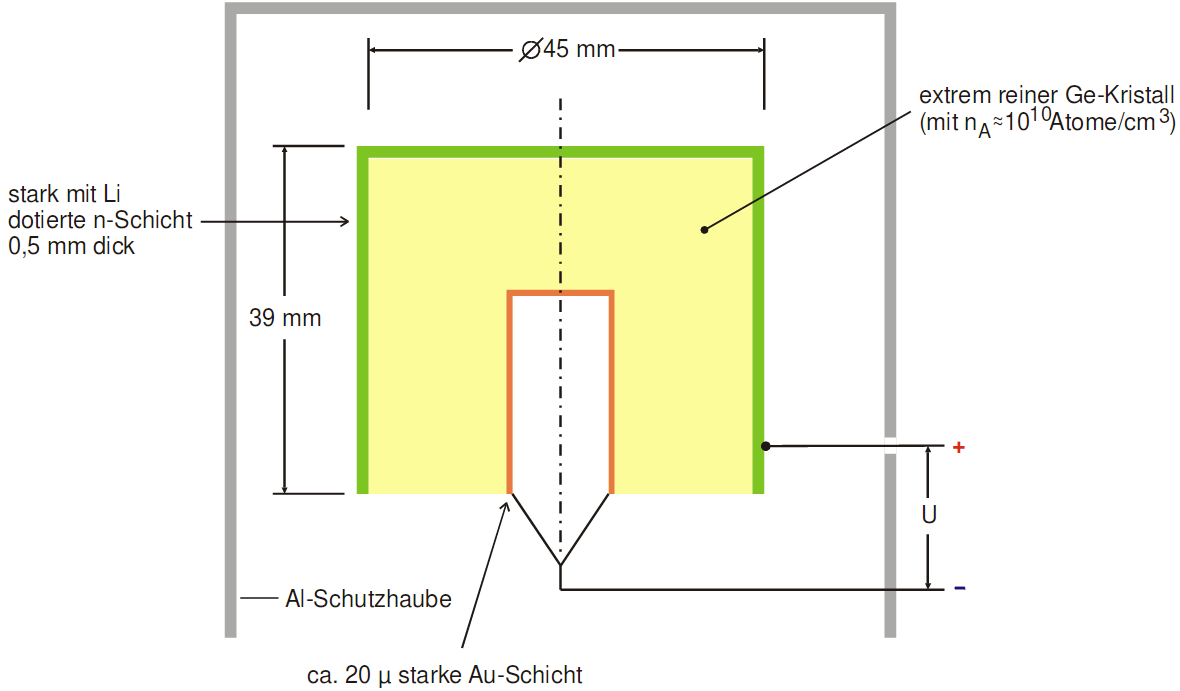
\includegraphics[width=0.9\linewidth]{Bilder/Germanium-Detektor.png}
  \caption{Schematischer Aufbau eines koaxialen Reinst-Germanium-Detektors \cite{V18}.}
  \label{fig:DetektorAufbau}
\end{figure}

\textbf{Vorverstärker:} \\
Die elektrische Ladungsmenge die in einem Germanium-Detektor erzeugt wird, kann durch elektrische Integration zu einem Spannungspegel umgewandelt werden. Dies wird mit Hilfe eines kapazitiv rückgekoppelten Operationsverstärkers durchgeführt. In Abbildung \eqref{fig:Vorverstärker} ist ein Vorverstärker skizziert. Für das Potential $U_\text{A}$ gilt
\begin{align}
  U_\text{A} = - \frac{1}{C_\text{K}} \int_{0}^{t_\text{s}} I(t) \text{d}t
\end{align}
\hfil {\footnotesize($t_\text{s}$ = Pulslänge der Sammelzeit)} \hfil \\
Wichtig für die Impulshöhenanalyse ist, dass der Integrationskondensator $C_\text{K}$ nach jedem Quantennachweis wieder entladen wird. Dies geschieht über eine optoelektrische Rückkopplung, "dabei wird nach jedem Impuls die Gate-Drain-Schicht des Eingangs-Feldeffekttransistors (FET) im Operationsverstärker von einer Lumineszenzdiode (LED) beleuchtet, sodass die Sperrschicht vorübergehend leitend wird und die Ladung auf $C_\text{K}$ darüber abfließen kann" (vgl. \cite[18]{V18}). Dieses Bauteil wird im Folgenden als $R_\text{K}$ eingezeichnet.

\begin{figure}[H]
  \centering
  \includegraphics[width=0.7\linewidth]{Bilder/Vorverstärker.png}
  \caption{Beschaltung eines Vorverstärkers im Reinst-Germanium-Detektor \cite{V18}.}
  \label{fig:Vorverstärker}
\end{figure}

\textbf{Hauptverstärker:} \\
Die Aufgabe des Hauptverstärkers ist es, die Spannungssignale auf maximal 10\,V zu normieren, da der Analog-Digital-Konverter (ADC) auf 10\,V genormt ist. Außerdem muss der Verstärker eine sehr hohe Linearität und Langzeitstabilität besitzten, weil die ADC's eine Auflösung von 8192 (13\,bit) besitzten. Auch muss die Bandbreite des Verstärkers geeignet gewählt werden, damit nur die wesentlichen Komponenten des Eingangssignals verstärkt werden. Diese Aufgabe übernehmen RC-Glieder als Hoch- und Tiefpassfilter. \\
Der Hauptverstärker wird häufig über ein RC-Glied an den Vorverstärker gekoppelt, siehe Abbildung \eqref{fig:Hauptverstärker}.

\begin{figure}[H]
	\centering
	\begin{subfigure}[t]{0.49\linewidth}
		\includegraphics[width=\textwidth]{Bilder/Hauptverstärker.png}
		\caption{Das RC-Glied zum koppeln des Vorverstärkers an den Hauptverstärker.}
		\label{fig:Hauptverstärker}
	\end{subfigure}
	\hfill
	\begin{subfigure}[t]{0.49\linewidth}
		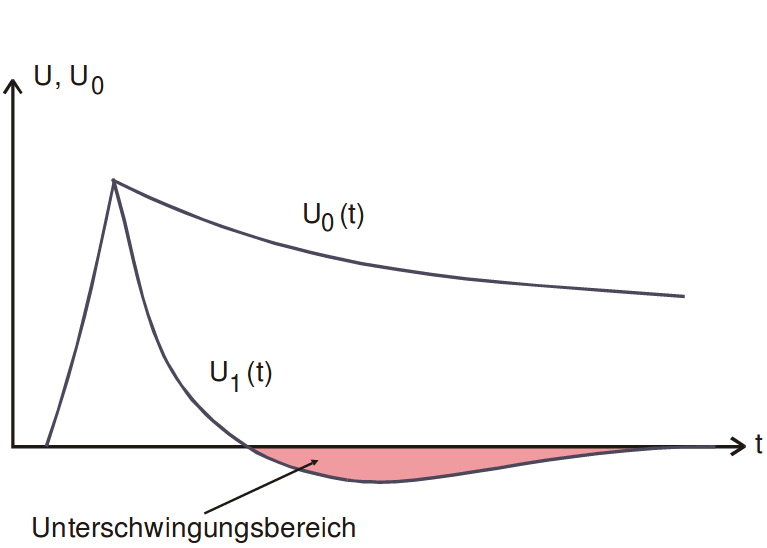
\includegraphics[width=\textwidth]{Bilder/Unterschwingung.png}
		\caption{Zeitlicher Spannungsverlauf von $U_0$ und $U_1$.}
		\label{fig:Unterschwingung}
	\end{subfigure}
  \caption{Das Koppelglied $R_1C_1$ und der zeitliche Verlauf der Signalspannung vor und nach dem Koppelglied \cite{V18}.}
\end{figure}

Dadurch werden Gleichspannungsdriften und Offsetspannungen nicht mit verstärkt. Allerdings kann dadurch eine Unterschwingung (siehe Abbildung \eqref{fig:Unterschwingung}) entstehen, weil die Abklingkonstanten $R_\text{K}C_\text{K}$ und $R_1C_1$ des Koppelgliedes verschieden sind. Dies kann verhindert werden, indem ein kleiner Teil der Gleichspannung vom Vorverstärker direkt zum Hauptverstärker geleitet wird ("Pole-Zero-Kompensation"). Am Ausgang des Hauptverstärkers kann ein ähnliches Problem auftreten. Dies wird aber über einen "Base-Line-Restorer" verhindert.

\textbf{Vielkanal-Analysator:} \\
Der Vielkanal-Analysator (VKA) besteht im Wesentlich aus dem ADC, einem Adressregister und einem Speicher. Diese dienen zum Speichern der Impulshöhen und der Häufigkeit der auftretenden Impulshöhen. In einem Diagramm kann nun die Impulshöhe bzw. die deponierte $\gamma$-Energie gegen die Häufigkeit aufgetragen werden. Aus diesem Diagramm können dann die Aktivität und die Energie bestimmt werden. \\



\section{Versuchsdurchführung}
Zu Beginn wird der Abstandshalter zwischen der Probe und dem Detektor vermessen, um den Raumwinkel bestimmen zu können. \\
Danach wird ein bekannter \isotope[152]{Eu}-Strahler in den Detektor eingesetzt. Dann wird die Messung gestartet, um den Messbereich der Energie festzulegen. Der Messbereich wird an einem signifikanten Doppelpeak bestimmt und soll von 0 bis 2500\,keV reichen. Sobald das Spektrum kalibriert ist wird eine 60 minütige Messung gestartet. \\
Nach dieser Messung werden noch drei weitere Spektren von \isotope[137]{Cs}, \isotope[133]{Ba} und einem unbekannten Mineral aufgenommen. Die Diagramme werden jeweils gespeichert und später ausgewertet.
